\documentclass{article}
\usepackage{tikz}
\usepackage[utf8]{inputenc}
\usepackage{enumitem}

\begin{document}

\section*{Aufgabe}
Folgendes Array enthält einen binären Max-Heap mit 10 Schlüsseln:
\[[\  98, 97, 41, 92, 51, 33, 39, 42, 63, 13\ ]\]
\begin{enumerate}[label=$\alph*)$]
    \item Zeichnen Sie diesen Heap.
    \item Fügen Sie in den Heap nacheinander die drei Schlüssel 86 38 47 ein
    und geben Sie den resultierenden Heap mit 13 Schlüsseln als Array
    an.
\end{enumerate}

\section*{Lösung}
\subsection*{a) Zeichnen Sie diesen Heap}
Der gegebene Max-Heap ist als Array dargestellt: 
\[[\  98, 97, 41, 92, 51, 33, 39, 42, 63, 13\ ]\]
Der Heap in Baumform sieht wie folgt aus:
\begin{center}
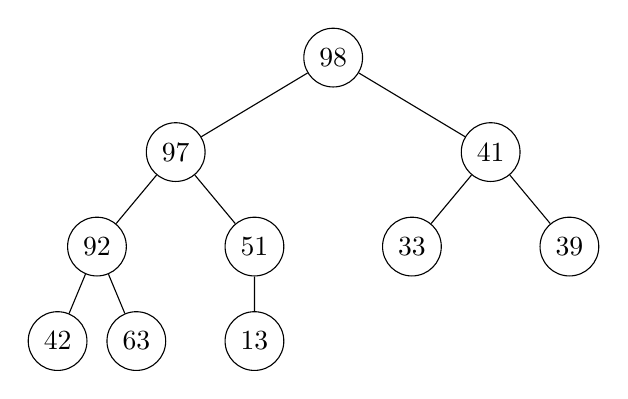
\begin{tikzpicture}[
  level distance=1.2cm,
  level 1/.style={sibling distance=4cm},
  level 2/.style={sibling distance=2cm},
  level 3/.style={sibling distance=1cm},
  every node/.style={circle, draw, minimum size=7mm}
]
\node {98}
    child {node {97}
        child {node {92}
            child {node {42}}
            child {node {63}}
        }
        child {node {51}
            child {node {13}}
        }
    }
    child {node {41}
        child {node {33}}
        child {node {39}}
    };
\end{tikzpicture}
\end{center}
In einem Array:
\begin{enumerate}[label=]
    \item \textbf{Ebene 1:} 98
    \item \textbf{Ebene 2:} 
    \begin{enumerate}[label=]
        \item 97
        \begin{enumerate}[label=]
            \item \textbf{Ebene 3:}
            \item 92
            \begin{enumerate}[label=]
                \item \textbf{Ebene 4:}
                \item 42
                \item 63
            \end{enumerate}
        \end{enumerate}
        \begin{enumerate}[label=]
            \item 51
            \begin{enumerate}[label=]
                \item 13
            \end{enumerate}
        \end{enumerate}
        \item 41
        \begin{enumerate}[label=]
            \item 33
            \item 39
        \end{enumerate}
    \end{enumerate}
\end{enumerate}
\newpage
\subsection*{b) Einfügen der Schlüssel 86, 38, und 47}
Die Schlüssel werden wie folgt eingefügt:
\begin{enumerate}[label=$b.\arabic*)$]
    \item \textbf{Einfügen von 86:} Der Schlüssel wird am Ende hinzugefügt und hochgehoben, um die Max-Heap-Eigenschaft zu bewahren.
    \item \textbf{Einfügen von 38:} Der Schlüssel wird am Ende hinzugefügt, aber keine weiteren Anpassungen sind notwendig.
    \item \textbf{Einfügen von 47:} Der Schlüssel wird am Ende hinzugefügt und hochgehoben, um die Max-Heap-Eigenschaft zu bewahren.
\end{enumerate}
Das resultierende Array lautet:
\[[\ 98, 97, 86, 92, 51, 41, 47, 42, 63, 13, 33, 38, 39\ ]\]
Der aktualisierte Heap in Baumform sieht wie folgt aus:
\begin{center}
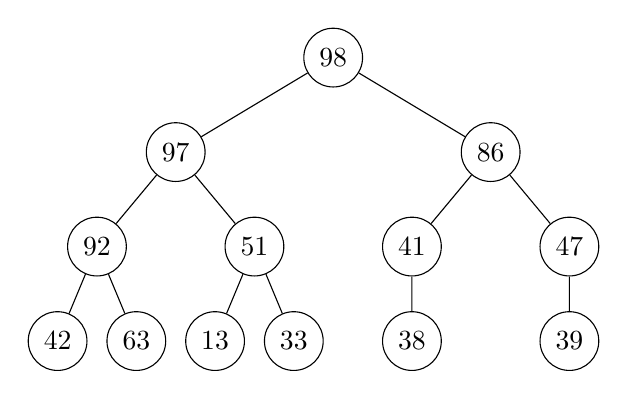
\begin{tikzpicture}[
  level distance=1.2cm,
  level 1/.style={sibling distance=4cm},
  level 2/.style={sibling distance=2cm},
  level 3/.style={sibling distance=1cm},
  every node/.style={circle, draw, minimum size=7mm}
]

\node {98}
    child {node {97}
        child {node {92}
            child {node {42}}
            child {node {63}}
        }
        child {node {51}
            child {node {13}}
            child {node {33}}
        }
    }
    child {node {86}
        child {node {41}
            child {node {38}}
        }
        child {node {47}
            child {node {39}}
        }
    };
\end{tikzpicture}
\end{center}

\end{document}
